

\documentclass[12pt]{article}
\usepackage{graphicx}
\usepackage{amsmath}
\usepackage{mathtools}
\usepackage{gensymb}
\usepackage{amssymb}

\newcommand{\mydet}[1]{\ensuremath{\begin{vmatrix}#1\end{vmatrix}}}
\providecommand{\brak}[1]{\ensuremath{\left(#1\right)}}
\providecommand{\norm}[1]{\left\lVert#1\right\rVert}
\newcommand{\solution}{\noindent \textbf{Solution: }}
\newcommand{\myvec}[1]{\ensuremath{\begin{pmatrix}#1\end{pmatrix}}}
\let\vec\mathbf

\begin{document}
\begin{center}
\textbf\large{CLASS 11 CHAPTER-11 \\ LINES}

\end{center}
\section*{Excercise 10.2}

Q18.$P(a,b)$ is the mid-point of the line segment between axes. Show that the equation of the line is $\frac{x}{a}+\frac{y}{b}=2$

\solution
Let
\begin{align}
	\vec{A}=x\vec{e_{1}}, \vec{B}=y\vec{e_{2}} \text{ and } \vec{P}=\myvec{a\\b}
\end{align}
where
\begin{align}
	\vec{e_{1}}=\myvec{1\\0} \text{ and } \vec{e_{2}}=\myvec{0\\1}
\end{align}
as shown in Figure \ref{fig:Fig1}
\begin{figure}[!h]
	\begin{center} 
	    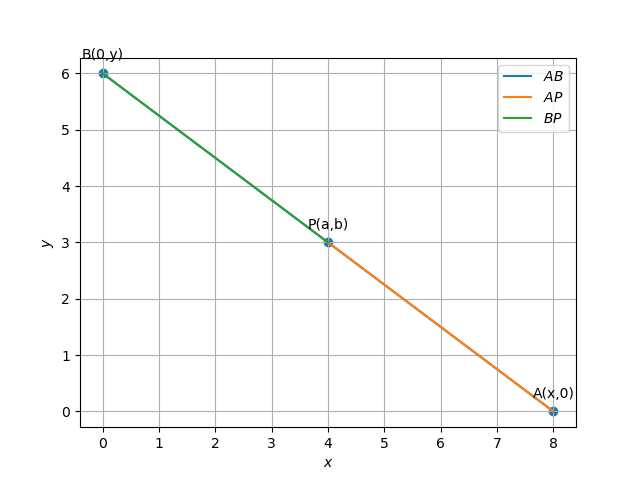
\includegraphics[width=\columnwidth]{figs/line1}
	\end{center}
\caption{}
\label{fig:Fig1}
\end{figure}

Now we know
\begin{align}
	\vec{P}&=\frac{\vec{A}+\vec{B}}{2}=\frac{x\vec{e_{1}}+y\vec{e_{2}}}{2}\\
	2\vec{P}&=x\vec{e_{1}}+y\vec{e_{2}}\\
	\vec{e_{1}}^{\top}\brak{2\vec{P}}&=\vec{e_{1}^{\top}}\brak{x\vec{e_{1}}+y\vec{e_{2}}}\\
					 &=x\\				 
	\vec{e_{2}}^{\top}\brak{2\vec{P}}&=\vec{e_{2}^{\top}}\brak{x\vec{e_{1}}+y\vec{e_{2}}}\\
					 &=y				 
\end{align}
So, from here we can say that
\begin{align}
	x&=2\vec{e_{1}}^{\top}\vec{P}=2a\\
	y&=2\vec{e_{2}}^{\top}\vec{P}=2b\\
	\vec{A} &= \myvec{2a\\0}\\
	\vec{B} &= \myvec{0\\2b}
\end{align}
Now direction vector is
\begin{align}
	\vec{m} &= \vec{A}-\vec{B}\\
		&= \myvec{2a\\-2b} = \myvec{1\\\frac{-b}{a}}
\end{align}
so normal vector is
\begin{align}
	\vec{n} = \myvec{1\\\frac{a}{b}}
\end{align}
So, the equation of line passing through $\vec{P}$
\begin{align}
	\vec{n}^{\top} \myvec{\vec{x}-\vec{P}} &= 0\\
	\myvec{1 & \frac{a}{b}}\myvec{\vec{x}-\myvec{a\\b}}&=0\\
	\myvec{1 & \frac{a}{b}}\vec{x}&=2a\\
	\myvec{1 & \frac{a}{b}}\myvec{x\\y}&=2a\\
	x+\frac{ay}{b}&=2a\\
	bx+ay&=2ab\\
	\frac{x}{a}+\frac{y}{b}&=2
\end{align}
Hence proved.


\end{document}
